\documentclass[border=10pt]{standalone}

\usepackage{fontspec}
\usepackage{xcolor}
\usepackage{tikz}
\usepackage{graphicx}

\setmainfont{Times New Roman}
\setsansfont{Arial}
\setmathrm{Arial}

\usetikzlibrary{arrows.meta}
\usetikzlibrary{shapes.misc}
\usetikzlibrary{positioning}
\usetikzlibrary{calc}

\tikzset{%
  base/.style = {rectangle, thick, draw=black!50, minimum width=2cm, minimum height=1cm, rounded corners=3pt},
  process/.style = {fill=white!10!green!20}
}

\begin{document}
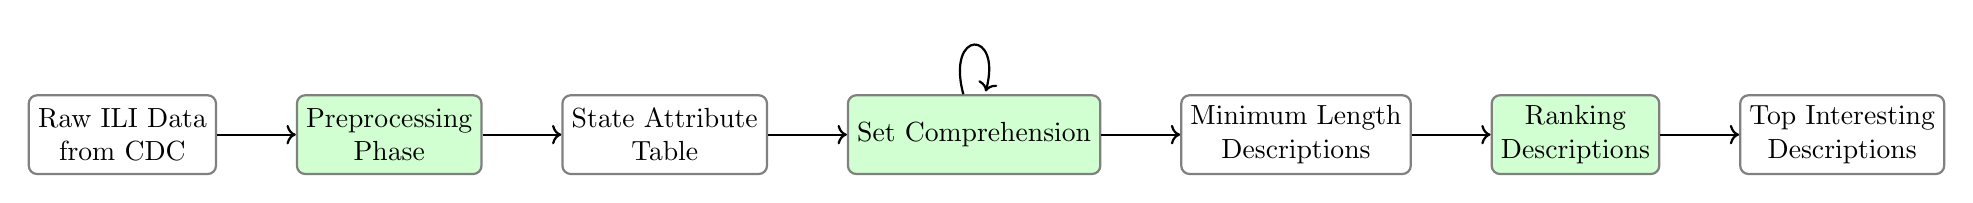
\begin{tikzpicture}[%
    node distance=1cm,
    every node/.style={base},
    thick,
    align=center]

  % Specification of nodes (position, etc.)
  \node (ili-data) {Raw ILI Data \\ from CDC};
  \node (preprocess) [process,right=of ili-data] {Preprocessing\\Phase};
  \node (state-attr) [right=of preprocess] {State Attribute\\Table};
  \node (setcomp) [process,right=of state-attr] {Set Comprehension};
  \node (mdl-desc) [right=of setcomp] {Minimum Length\\Descriptions};
  \node (rankpatt) [process, right=of mdl-desc] {Ranking \\Descriptions};
  \node (top-mdl-desc) [right= of rankpatt] {Top Interesting \\ Descriptions};
  

  \draw[->] (ili-data) -- (preprocess);
  \draw[->] (preprocess) -- (state-attr);
  \draw[->] (state-attr) -- (setcomp);
  \draw[->] (setcomp) edge[loop above] (setcomp);
  \draw[->] (setcomp) -- (mdl-desc);
  \draw[->] (mdl-desc) -- (rankpatt);
  \draw[->] (rankpatt) -- (top-mdl-desc);
\end{tikzpicture}
\end{document}
